\chapter{Overview}
\label{storage}

\section{Components}
\label{storage:components}

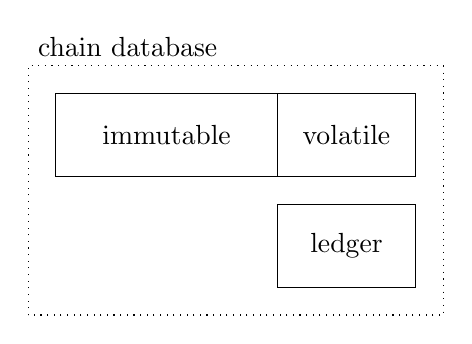
\begin{tikzpicture}
\draw [dotted]
     (-50pt, -65pt)
  -- ++(0, 90pt) node[above right] {chain database}
  -- ++(150pt, 0)
  -- ++(0, -90pt)
  -- cycle;
\node [draw, shape=rectangle, minimum width=80pt, minimum height=30pt] at (0,0)  {immutable};
\node [draw, shape=rectangle, minimum width=50pt, minimum height=30pt] at (65pt, 0)  {volatile};
\node [draw, shape=rectangle, minimum width=50pt, minimum height=30pt] at (65pt, - 40pt) {ledger};
\end{tikzpicture}

Discuss the immutable/volatile split (we reference this section for that).

\section{In memory}
\label{storage:inmemory}

TODO: After we discussed the overview, we should give an overview of everything
we store in memory in any component, so that we have a better understanding of
memory usage of the chain DB as a whole.

\subsection{Chain fragments}
\label{storage:fragments}

\subsection{Extended ledger state}
\label{storage:extledgerstate}
\label{storage:headerstate}

TODO: Is there a more natural place to talk about this? Introducing the
header state when introducing the storage layer does not feel quite right.
The storage layer might be storing the header state, but that doesn't
explain its existence.

ChainDepState, (ChainIndepState), LedgerState, ExtLedgerState
